%!TEX root = ../Master.tex

\section{Particle Filters}

Particle Filter (PF) is another method for estimating the state of at system. As opposed to the Histogram Filter which is discrete in the state space and multimodal and Kalman Filter which is continuous in the state space but unimodal, the PF is continuous in the state space but also multimodel in its posterior belief. However, in robotics all of the methods are only approximations of the actual system state.\\

PF can be used to perform global localization of a robot, given a map of the environment in which the robot resides at some unknown location. The robot acquires distance measurement to objects in its vicinity, then particles will be spread out at random locations on the map which represents the robot as if it was located at these locations. That is, each particle is a discrete guess about the robots location, which consists of coordinates and a heading. Each particle will then acquire distance measurement to objects in their vicinity and by comparing these measurement with the actual robots measurement, an estimation of the robots location is obtained as the particles who's measurements best resembles the actual robots measurement.\\
However, similar measurement can probably be obtained at different locations on a particular map, and therefore the robot needs to move around the in environment and acquire new measurement. At some point in time as the robots moves around, it acquires new measurement and particles which are must consistent with the measurement have a higher probability of being resampled. As a result, locations with a high probability will collect more particles and will therefore be more representative of the robots posterior belief. When all of the particles are clustered at a single location, this location will (hopefully) be the robots actual location.\\

To help summarize the operations of the PF, \autoref{fig:pf_ex1} shows a initial belief where the robot is totally uncertain about its location, which is represented by a uniform distribution of the particles of which there are several thousands in this example. The blue lines represent the distance measurements obtained by the robot.

\begin{figure}[H]
\centering
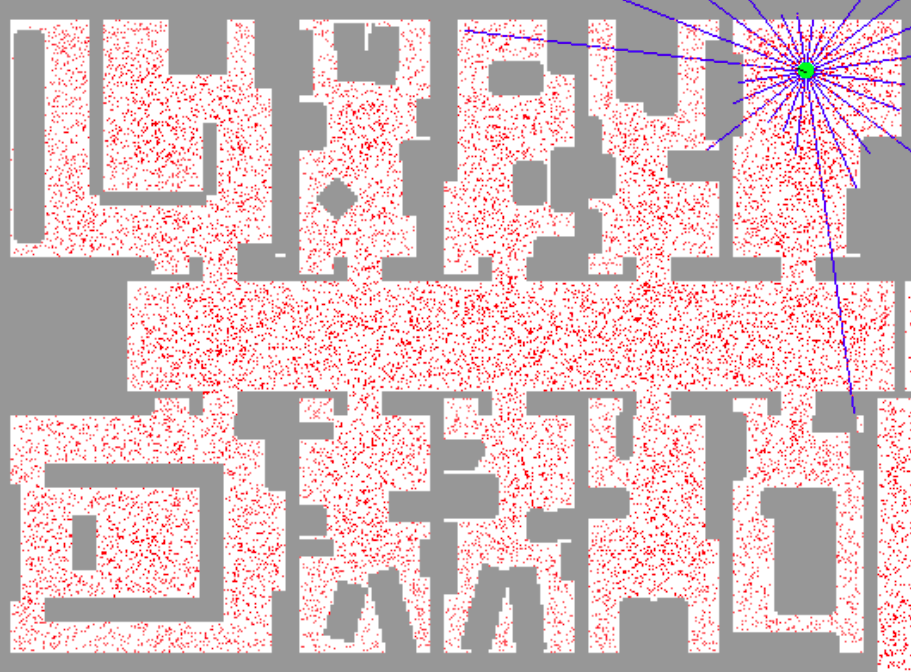
\includegraphics[scale=0.45]{images/particlefilter1}
\caption{Particle Filter initial posterior belief}
\label{fig:pf_ex1}
\end{figure}

Next, \autoref{fig:pf_ex2} shows the robot after having moved around in the environment and acquired new measurements and resampled the particles. This have let to some particles being eliminated and others surviving. The surviving particles are thoughts who are must consistent with the robots measurement. At this point it is still very uncertain where the robot resides.

\begin{figure}[H]
\centering
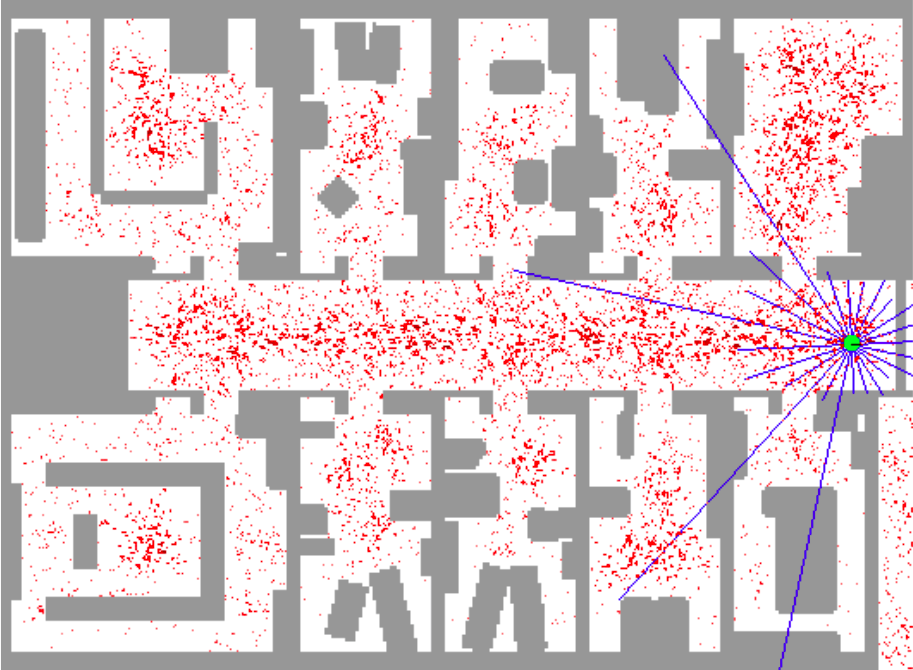
\includegraphics[scale=0.45]{images/particlefilter2}
\caption{Particle Filter posterior belief after x timesteps}
\label{fig:pf_ex2}
\end{figure}

\begin{figure}[H]
\centering
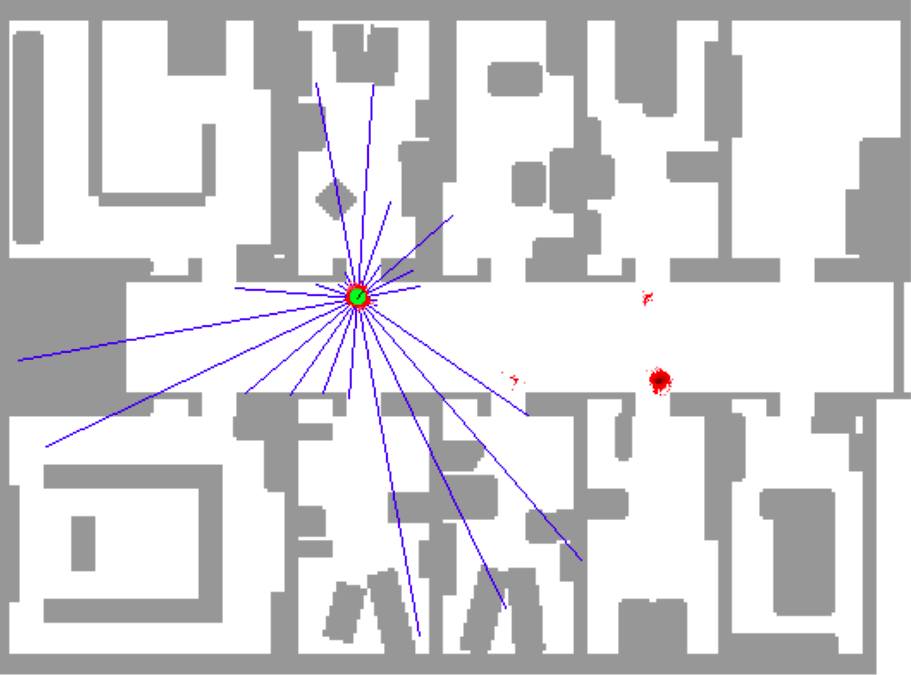
\includegraphics[scale=0.45]{images/particlefilter3}
\caption{Particle Filter posterior belief with two clusters because of symmetric in the map}
\label{fig:pf_ex3}
\end{figure}